\chapter{DNS Rebinding}

DNS rebinding is a computer attack, by which an attacker subverts the
same-origin policy of browsers, this can effectively convert the browser into
an open network proxy~\cite{jackson2009protecting}.

\vspace{0.5cm}

\begin{figure}[H]
\begin{center}
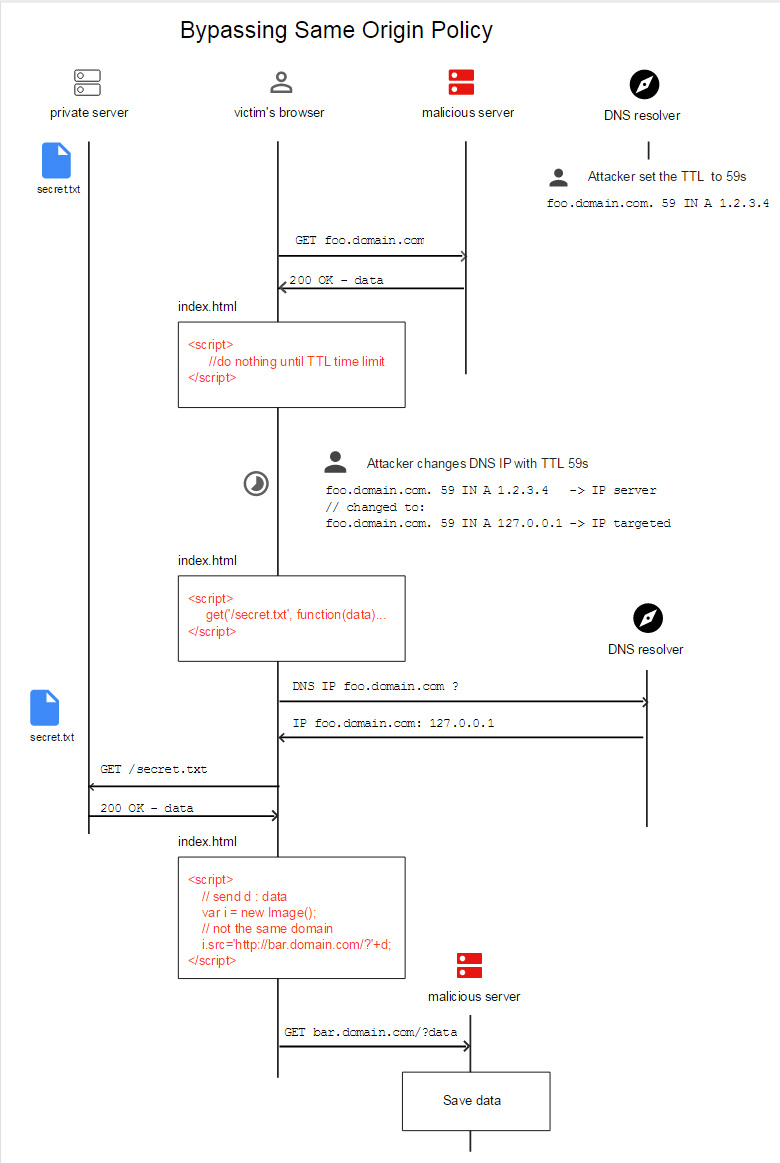
\includegraphics[width=0.59\textwidth,keepaspectratio]
{img/dnsrebindingflow.jpg}
	\caption{DNS Rebinding Flow Diagram (Taken from~\cite{vulnsec})}
\end{center}
\end{figure}

\vspace{0.5cm}

DNS Rebinding works by alternating DNS responses between the attacker server IP
and the target machine IP.

For example, an attacker could register a domain name
\texttt{rebind.attacker.com} and set up the DNS responses to alternate between
the legitimate server (e.g. \texttt{10.0.1.55}) and the target server (e.g.
\texttt{127.0.0.1}).

When a user attempts to connect to \texttt{rebind.attacker.com}, assuming the
DNS currently resolves to the attacker server (\texttt{10.0.1.55}), the
attacker can serve specially crafted JavaScript that continually make HTTP
requests waiting for the DNS to resolve to the target IP (\texttt{127.0.0.1}).
At this point the attacker script can make arbitrary HTTP requests which appear
to originate from \texttt{127.0.0.1} effectively bypassing the SOP.

If an application relies on the SOP only for security, and does not explicitly
check Host headers, this can constitute to a security vulnerability. Our
implementation attacks a (now-patched) vulnerable version on the popular
Transmission~\cite{transmission} torrent client, which leads arbitrary code
execution (See~\S\ref{implementation} for details).

\section{Types of DNS Rebinding}

There are multiple ways to implement ways to implement DNS rebinding in order
to enable DNS rebinding attacks. Here we summarise two ways: Multiple A
Records, and Time-Varying.

\subsection{Multiple A Records}

When a web browser resolves external host names, the DNS server can respond
with A records (usually two) which contain the IP address information of
the host. Jackson et al.~\cite{jackson2009protecting} describe a DNS rebinding
attack using multiple A records using the following scenario:

\begin{enumerate}
\item{"The user's browser visits a malicious Web site, http://attacker.com/,
that
contains a Java applet. The attacker's DNS server (which is authoritative
for attacker.com) responds with two A records: one that contains the IP
address of the attacker's Web server and another that contains the IP address
of the target's Web server. The JVM chooses one of these IP addresses,
typically the first, opens a socket, and retrieves the applet."}
\item{"The browser runs the attacker's applet, which requests that the JVM open
a socket to the target's IP address. The JVM opens the socket because the
target's IP address is contained in the DNS response for attacker.com."}
\end{enumerate}

\subsection{Time-Varying}

A DNS rebinding attack using Time-Varying DNS involves an external host name
being bound to a very short TTL (Time To Live). After rebinding the specified
external host name to a target IP address, a HTML document located on the
attacker's server contains a script which sends an XMLHttpRequest which
connects to another URL on the external host name, ultimately resolving to
the target server.

\vspace{0.5cm}

This works as when the XMLHttpRequest is issued, the browser issues another DNS
query to the external host name, due to its DNS cache expiring. The attacker's
DNS server responds with a singular A record which binds the attacker's
external
host name to the target IP address with a short TTL. Because of this second
DNS query, which was issued to the same external host name as the original one
containing the attacker's script, the browser sends a HTTP response to the
script, which then sends data back to the attacker's server.

\section{Motives}

The primary objective of an attacker performing a DNS rebinding attack is to
breach a target's private network. Through the breach, an attacker can employ
the attack to perform malicious activities from the target machine, including:
\begin{itemize}
	\item{Mass Email Spamming}
\item{Implementing a Remote Administration Tool (RAT) into the target machine}
	\item{Distributed Denial-of-Service (DDoS) Attacks}
\end{itemize}
